\chapter{My commitments to the project}

I aim to generalize this writing and be less specific about the exact project we are working on, so the following experiences can be transferred to other fields of otherwise non related studies.
Basically our task was a simple classification problem for time samples of various length.
My task was not just to try out famous Machine Learning concepts which \textit{may} work, but to support our research group with the necessary backend of the experiments carried out, and to integrate different results in the final unified model.

\paragraph{Environment.}
For doing so I decided to use TensorFlow environment, in which I had previous experience, i.e.\ in building semantic analyzer for movie dialogs, image classifiers, and text generation for chatbots, image generation using Generative Adversarial Networks etc.
For our project we started by applying different previously proven to be succesful feature extraction methods, and for introducing Deep Learning we wanted to improve our progress by building on top of these features.
So in the first step I had to break down the recent DL architectures I wanted to use to basic modules.
When reimplementing them I paid attention to make spaceholders or entry points for every possible external features my colleagues developed.

Entry points at different level of processing the input can be categorized as the following:
- Variable length features (i.e. output of filters).
- Fixed representation features (i.e. variability indices, frequency domain components).
- Suggestions for classes (i.e. external classifier suggestion)

Also, to improve the model's efficiency I applied queues after different entry points to make mini-batch processing available, by filling these queues independently in mutliple threads, so the network trainer do not have to wait for these external sources to finish their processes to update the network's weights.

\paragraph{Data standardization.}
The biggest obstacles at first sight in using TensorFlow are the Tensors and the (control) Flow itself. In order to deploy a model we have to first assemble its computational graph, which will be compiled at run-time so it can be fed with real NumPy arrays and evaluated in the most efficient way relying on the TensorFlow backend.

Knowing that any time we feed values in, and retreive values from Tensors the whole process has to switch back and forth between C++/CUDA backend and the Python interface, which in case of large arrays is computationally expensive, and possibly collapse the parallel processes to sequential evaluation causing unnecessary run-time overhead, making TensorFlow seemingly inefficient.
In order to achieve best performance we have decrease the number of python API calls of Tensor evaluation, to let the backend order its computations in one run.

Special case of reducing calls is to discard the notorius use of placeholders~\cite{noauthor_performance_nodate, noauthor_tensorflow:_nodate}, and introduce Queues to the model.

TensorFlow comes with a handful of convenience functions and wrappers which can handle data loading and preprocessing in parallel threads, controlled by a native thread coordinator.

These operators can be built in the graph without actually loading the data, and provide Tensor outputs which instead of placeholders will feed the network automatically on evaluation, so we can forget the \textit{feed dict}.
By using queues we can ensure that the main training process is running continously by chopping minibatches off the queues' front while new samples are fed back to the other end, possibly on different devices and multiple threads.
As a result the main process will not starve on input data, neither will be continously interrupted by Python calls to simply just transfer values from the API to the backend.

For the reasons above I prepared a \textit{writer.py} script that takes our raw data files, reads them into memory and write them out in a single file in the suggested file format, \textit{.TFRecord}.
These files can be managed more easily, preserve the sufficient data in a compact way~\cite{noauthor_tfrecords_nodate}, and the most important part, they can be automatically transformed into Tensors.

To make our experiments standardized, we first separated a train and a test set from the original data in 80-20 ratio, and due to unbalanced entries class representation, I wrote and augmentation script to create an evenly sampled pre-training set with a disjunct train and validation set (80-20), in order to prevent the model from learning a single answer for every sample.

\paragraph{Digital Filter.}
Since our original approach was built upon modified Pan Tompkins filtering method~\cite{pan1985real}.
When we refactored our code base to use TensorFlow, we approached a great obstacle: there was no previous work involving filters.
While in SciPy we could reproduce the same results of the original MatLab code~\cite{noauthor_complete_nodate}, the above mentioned problem of feeding external values instead of integrating the process in the computational graph was apparent again.
We had to decide whether we pre-process all sample before writing the 'TFRecords' files keeping the heavy computing outside of our model, or implement the repeatedly used 'filtfilt' operation, and rewrite the method completely using abstract native TensorFlow Tensors and Op nodes.

Considering that we have to deploy the algorithm in real time inference application, we choose the latter.
As a first step, my colleagues reimplemented the method using NumPy, that I used as a template to follow while writing a new basic TF operator called 'lfilt'.
I paid attention to keep the TF policy which is that operators borrowed from SciPy and NumPy should be transparent by function call signature, and the output should behave the same way as in the original implementation.


- FeedBack filter components:   $A = a_0, a_1, a_2 \dots a_M$, where $a_0 = 0$ by definition
- FeedForward filter components:   $B = b_0, b_1, b_2 \dots b_N$

\begin{lstlisting}[language=Python]
# Lfilt operation definition at time step `t`
y(t) = x(t)*b(0) + x(t-1)*b(1) + x(t-2)*b(2) ... x(t-M)*b(N)
                       - y(t-1)*a(1) - y(t-2)*a(2) ... y(t-N)*a(M)
\end{lstlisting}

$$
y_t = \sum_{i=0}^{N} x_{t-i} \cdot b_{i} - \sum_{i=1}^{M} y_{t-i} \cdot a_{i}
$$


\begin{lstlisting}[language=Python]
y(t) = x[t-N : t] * b[::-1] - y[t-M : t-1] * a[::-1]
\end{lstlisting}


for faster computation let $s$ be $s := x \ast b$, where $\ast$ is the convolution operator. This can be evaluated previusly at once since all values of $x$ is known at computation time

\begin{lstlisting}[language=Python]
y(t) = s[t] - y[y-t : t-1] * a[::-1]
\end{lstlisting}

As in the SciPy source code we can see~\cite{noauthor_scipy/scipy_nodate}, on lfilt calls both $A$ and $B$ are expected to include the $0^{th}$ parameter as well, which in the feedback operator's case will mean that in the exact computation we have to normalize both $A$ and $B$ by $A_0$ and leave out the $0^{th}$ component from $A$, since it is the corresponding constant of the current $y_t$ value.

\paragraph{Visualization.}
We always have to keep track, of what we have tried before, and after dozens of runs of experiments it is only up to us what we logged, and how well can we remember.
To make a decision on future steps in the project it is always useful if we can avoid crawling through a messy git history to find the actual train scripts we wrote, then start to extract the hyperparameters from the code - it uses up a tremendous time, and chances of missing something is very high.

To make debugging, optimization, and workgroup meetings productive, I used TensorBoard, that is able to read native TensorFlow log or \textit{summary} files and automatically turns them into spectacular graphs (see Figure \ref{fig:tf-graph} and \ref{fig:hist}), and quantitative metrics (see Figure \ref{fig:tf-score}).
The more explicit name and variable scopes we include in our code the more detailed the resulting graph and scorings will be.

\begin{figure}[h]
  \centering
  \includegraphics[width=\textwidth]{tf-graph}
  \caption{Left: Inner structure of a FCN. Right: The \textit{Confusion Matrix} operator is build using elementary TensorFlow operations.}
  \label{fig:tf-graph}
\end{figure}

\begin{figure}[h]
  \centering
  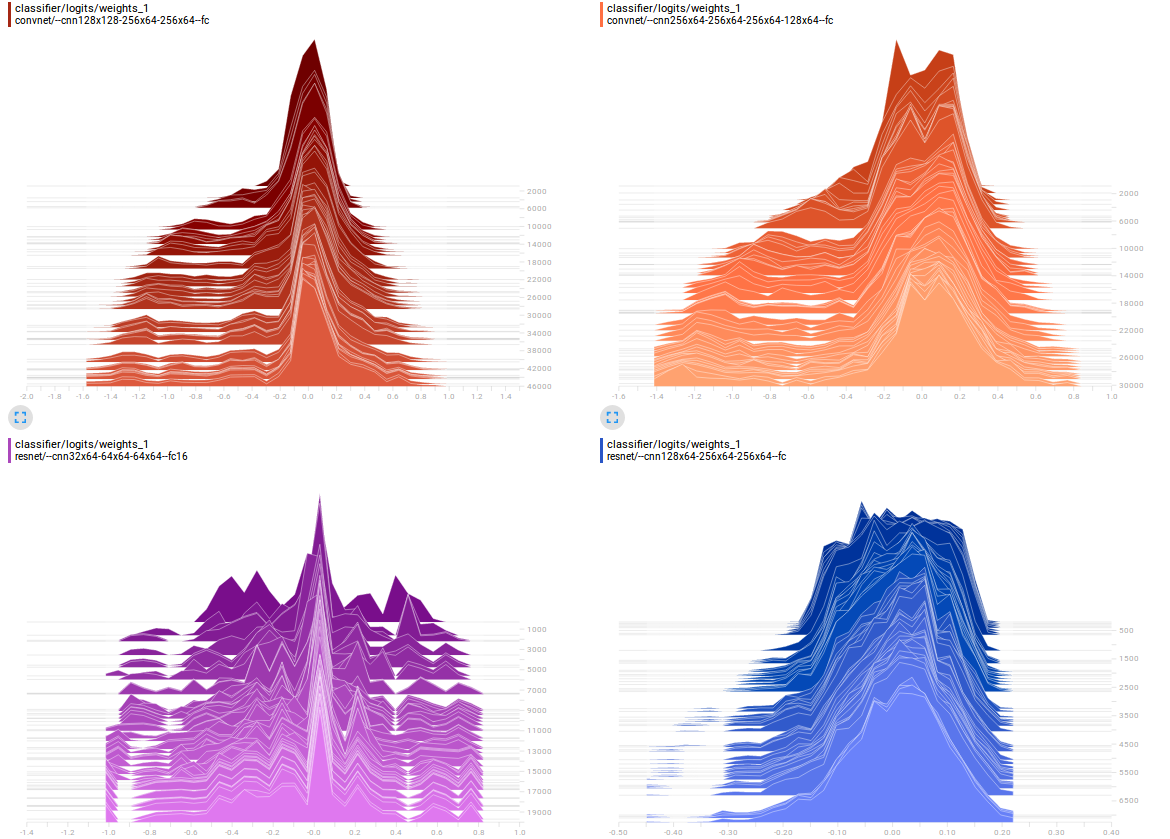
\includegraphics[width=\textwidth]{hist}
  \caption{Using histograms we can keep track of our model's progress during the training session. We may look for local pikes in the distribution of the layers' weights, or biasing toward a specific mean through time.}
  \label{fig:hist}
\end{figure}

\begin{figure}[h]
  \centering
  \begin{floatrow}
    \ffigbox[\FBwidth]{\caption{Performance test of Deep Residual networks}}{%
      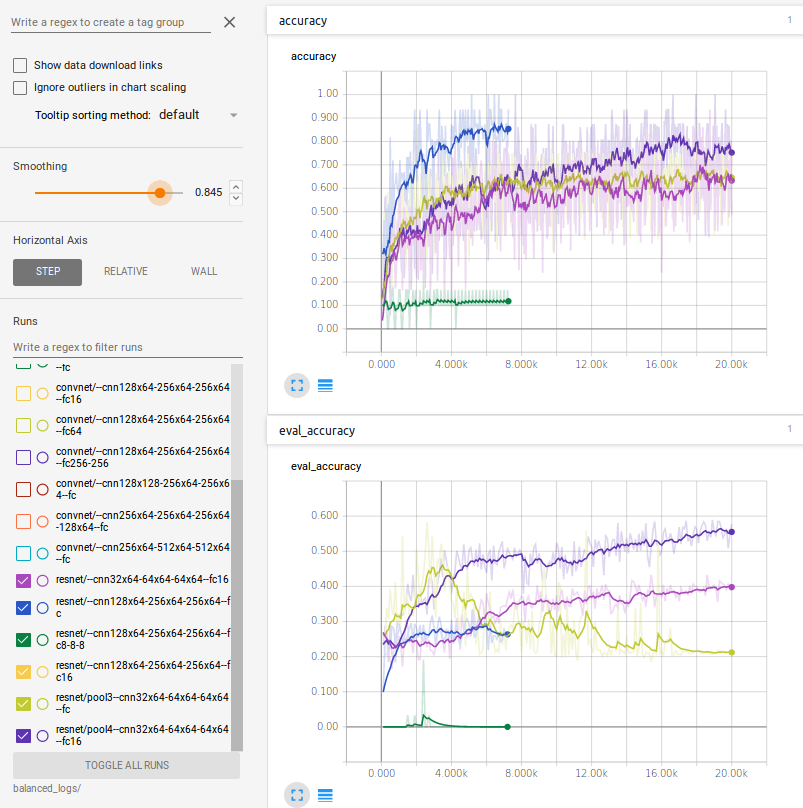
\includegraphics[width=.48\textwidth]{resnet-overall}
    }
    \ffigbox[\FBwidth]{\caption{Performance of Fully Convolutional networks}}{
      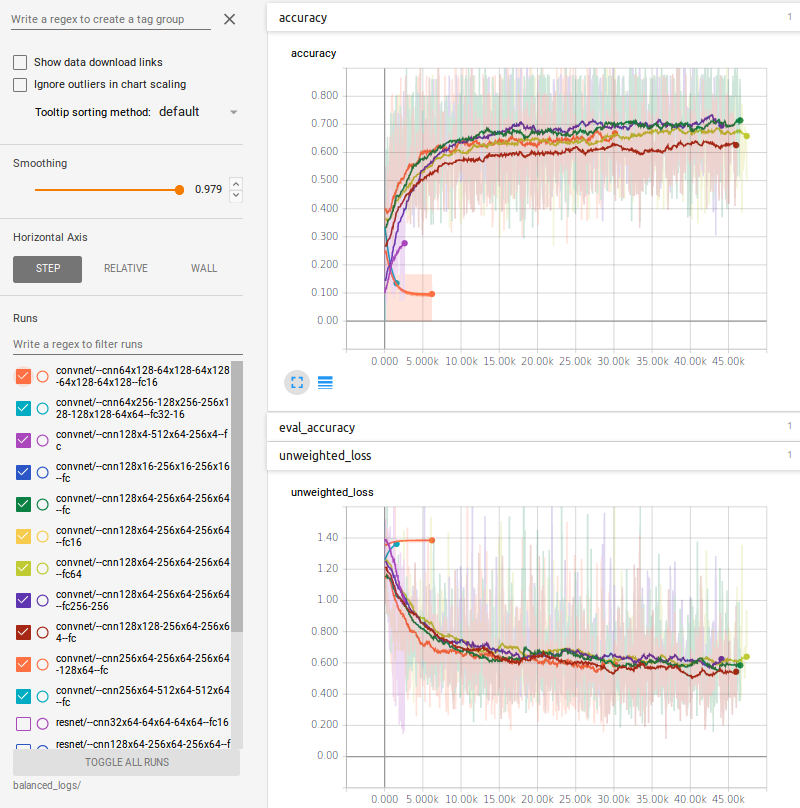
\includegraphics[width=.48\textwidth]{convnet-overall}
    }
  \end{floatrow}
  \label{fig:tf-score}
\end{figure}

By utilizing TensorBoard we boosted our progress, because we could easily determine if a training should be stopped because the network collapsed, track down which layer was causing this failure by investigating the forward and backward pass of activations and gradients, the distribution of the models variables grouped by layers - all in all whether an experiment branch should be further investigated or not.

\paragraph{Fast prototyping.}
To make our experiments easily reproducible I refactored our network modules to be able to build themselves by just simply using a few high level hyperparameters, just like as number of internal layers, capacity, reduction factor (av/max pooling), etc. and made a template \texttt{.json} file which held these prototype variables, allowing us to use the same training script to build and train a wide variety of different architectures while saving and logging them in high detail to separate directories.

When servers with multiple GPUs are available, we can also boost our fine-tuning phase, with running trainings on parallel threads.
By default a single TensorFlow session allocates the whole GPU source, even if the graph is not able to use but a single unit.
So for parallel tests, I wrote a shell program with which we can launch the training with different parameters, automatically reserving the required devices to each training and restricting it from interfering in other processes.
